\documentclass[english]{article}

\usepackage{babel}
\usepackage{graphicx}
\usepackage{times}
\usepackage{pifont}
\usepackage[margin=1in]{geometry}
\usepackage{eurosym}
\usepackage{fancyhdr}
\usepackage[hidelinks]{hyperref}
\usepackage{float}

\pagestyle{fancy}
\fancyhf{}


%HEADER
%**************************************************************************************
\pagestyle{fancy}
\fancyhf{}
%**************************************************************************************
\lhead{Database}		 	 
\rhead{Pricelizer} 
\lfoot{\today}
\cfoot{\thepage}
\rfoot{Alexey Tukalo}
%**************************************************************************************

\date{}
\setlength\parindent{0pt}

\begin{document}

\title{\vspace{3in}Database\\
\small Pricelizer\\
}

\nopagebreak
\maketitle


\vspace{4in}



\date{\today}
\thispagestyle{empty}

\newpage
\setcounter{page}{1}
\setcounter{tocdepth}{2}

\newpage

%MAIN CONTENT ******************************************************************************************************************


Our server is running inside siteground.com hosting, so to get an access to the database first of all we should login ourself to the siteground.com.
You can see the login field on the fig. 1.

\begin{figure}[H]
\centerline{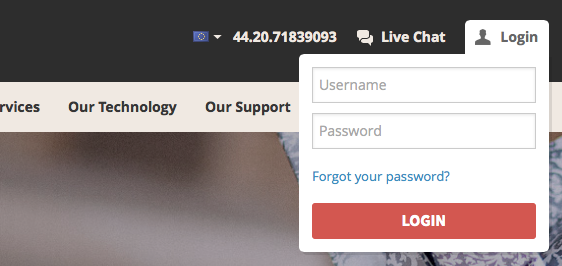
\includegraphics[scale=0.35]{PDatabase/sg}}
\caption{Login filed}
\end{figure}

After that you need to get an access to cPanel, for it you have to press the button (figure 2) and enter the login and password for cPanel at the login page.
\begin{figure}[H]
\centerline{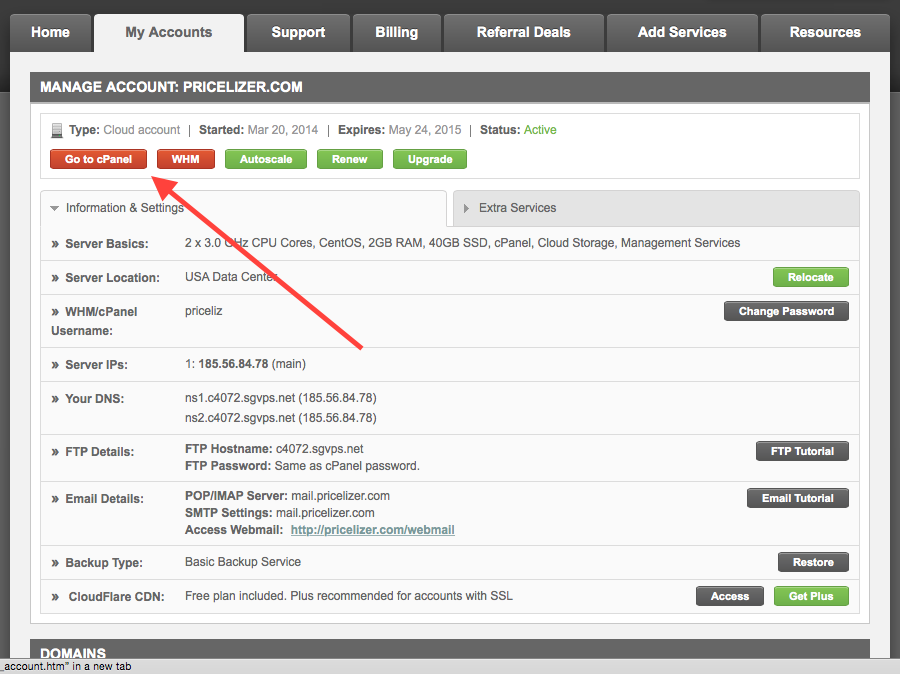
\includegraphics[scale=0.35]{PDatabase/cp}}
\caption{cPanel button}
\end{figure}

You can find the database tools(fig. 4) if you'll scroll down on the main page of cPanel until database section 
(fig. 3).
\begin{figure}[H]
\centerline{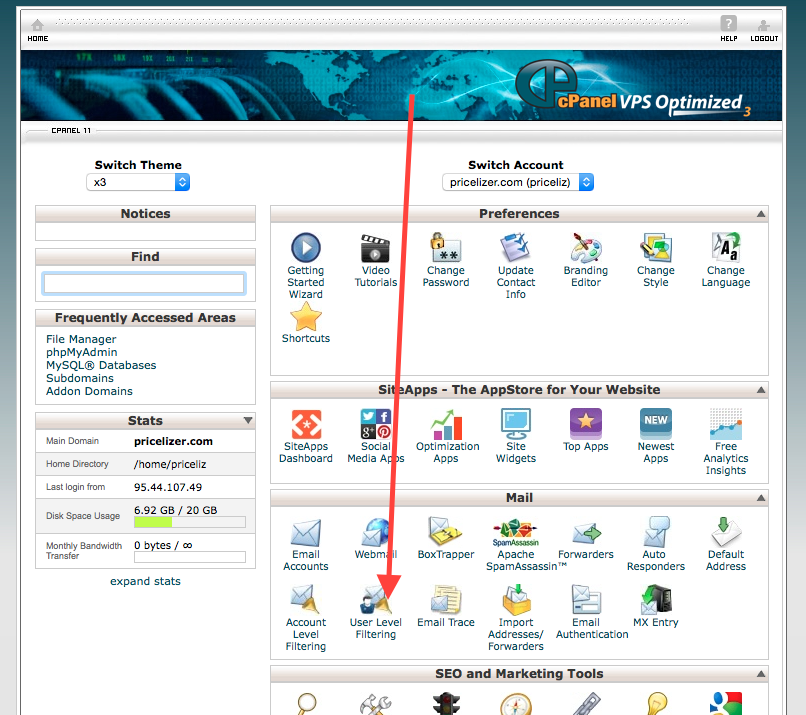
\includegraphics[scale=0.35]{PDatabase/mcp}}
\caption{Main page of cPanel}
\end{figure}
\begin{figure}[H]
\centerline{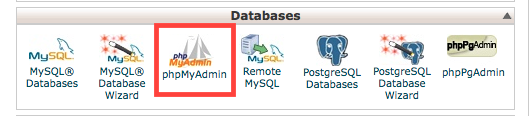
\includegraphics[scale=0.5]{PDatabase/db}}
\caption{Database section}
\end{figure}

We are running MySQL database, so you can get full access to the tool via phpMyAdmin (fig. 5).
\begin{figure}[H]
\centerline{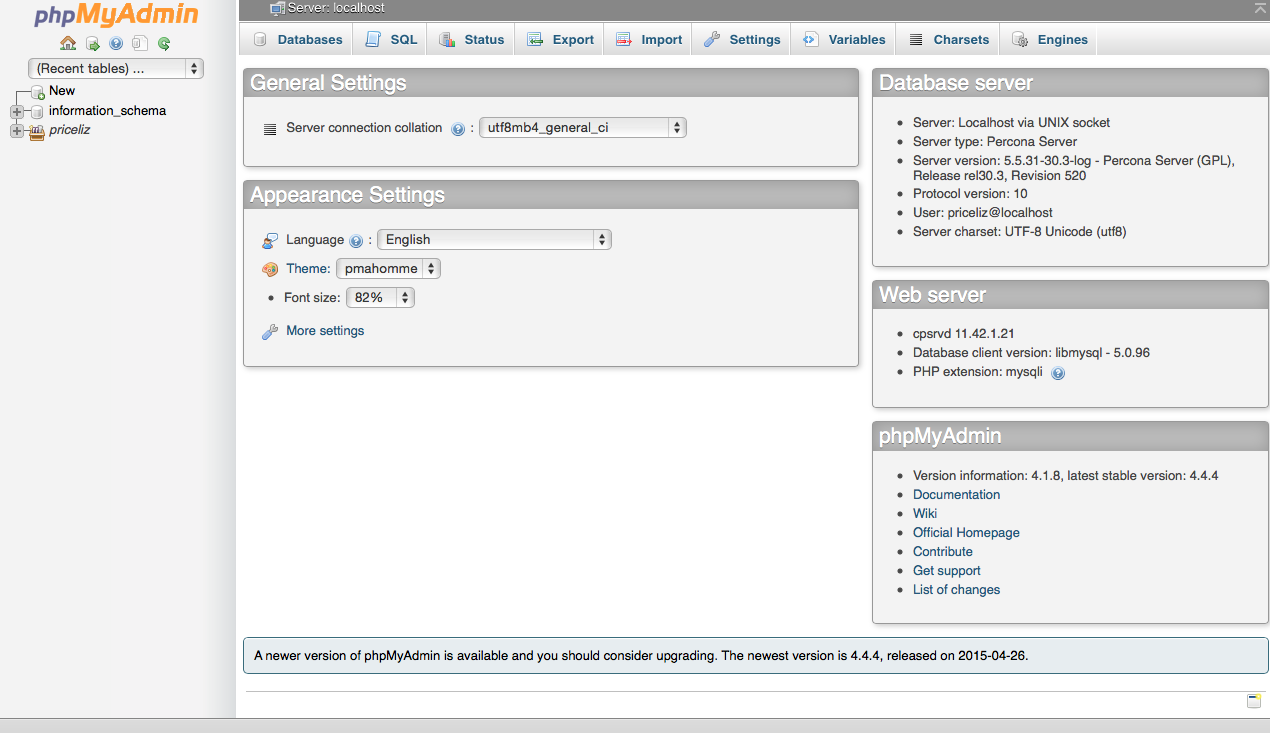
\includegraphics[scale=0.25]{PDatabase/dbm}}
\caption{phpMyAdmin main page}
\end{figure}



\end{document}
